\subsection{Comparison of Public and Self-Generated Datasets}
% warum ist der Vergleich wichige? zwischen den beiden Datensätzen
The paper \textit{Enhancing EV Charging Station Security Using a Multi-dimensional Dataset}~\cite{EV_Security} and my work pursue the same goal: detecting anomalies through the analysis of HCP and kernel events. Therefore, it is essential to compare the underlying datasets on which the machine learning algorithms are trained. Such a comparison enables validation of the respective approaches and helps determine whether the results can be generalized.

% Beschreibung der Datensaätze: Herkunft Umfang, Struktur, Einschrnänkunen
We tried to get as close as possible to the environment of the paper \textit{Enhancing EV Charging Station Security Using a Multi-dimensional Dataset}\\
\begin{figure}[H]
  \centering
  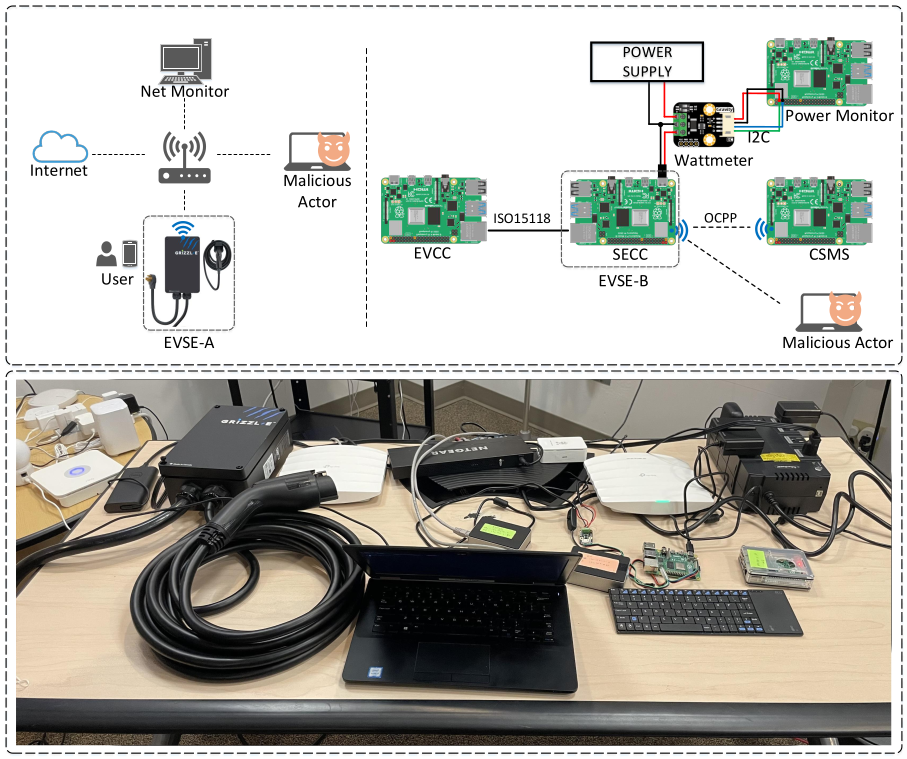
\includegraphics[width=0.7\textwidth]{pics/setup_public_paper.png}
  \caption{setup EV Charing Station from \cite{EV_Security}}
  \label{fig:setup_public_paper}
\end{figure}
We also used a Raspberry Pi to represent the EVSE-B and employed a wattmeter to monitor power consumption. The combination of HCP events, kernel events, and power consumption measurements will be discussed in future work. As mentioned in Chapter~\texttt{Data Sources for EVSE Anomaly Detection}, we also used the \texttt{perf} tool to monitor the various events.\\
\\
Therefore, we are able to observe approximately 900 events—similar to the comparison dataset. The complete observation period spans from \texttt{2025-07-22T18:00:00} to \texttt{2025-07-23T12:52:10}, with a sampling interval of 10 seconds, resulting in approximately 8,000 data rows with 905 columns. There are no missing (NaN) values in the dataset, and all measurements were collected using the \texttt{perf} tool, producing logically consistent outputs, as described in the chapter \textit{Data Sources for EVSE Anomaly Detection}.\\
Features that are distributed across multiple CPU cores (e.g., \texttt{cpu=0,1,2,3}) are aggregated using appropriate \texttt{perf} flags. This prevents data loss and reduces the number of distinct features, aligning the dataset structure more closely with that of the comparison \texttt{CICEVSE2024} dataset.\\
The \texttt{CICEVSE2024} dataset consists of the same 905 event types and comprises approximately 8,500 rows. Timestamps are recorded as floating-point numbers representing the time of each measurement. The data was collected using the \texttt{perf} tool, ensuring high precision and consistency across all recorded events.\\
Out of the entire dataset, only four rows contain \texttt{NaN} values across all features. These rows can be considered outliers or errors and can easily be excluded during preprocessing. To ensure comparability with the reference dataset, features distributed across multiple CPU cores (e.g., \texttt{cpu=0,1,2,3}) were aggregated using appropriate \texttt{perf} flags. While it is not explicitly stated in the documentation of the \texttt{CICEVSE2024} dataset whether a similar aggregation was performed, the reduced feature dimensionality suggests that such a step may have been taken. Therefore, this approach was adopted in our dataset to align the structure and avoid data duplication.
% Visulaisierung der Unterschiede
\begin{figure}[H]
  \centering
  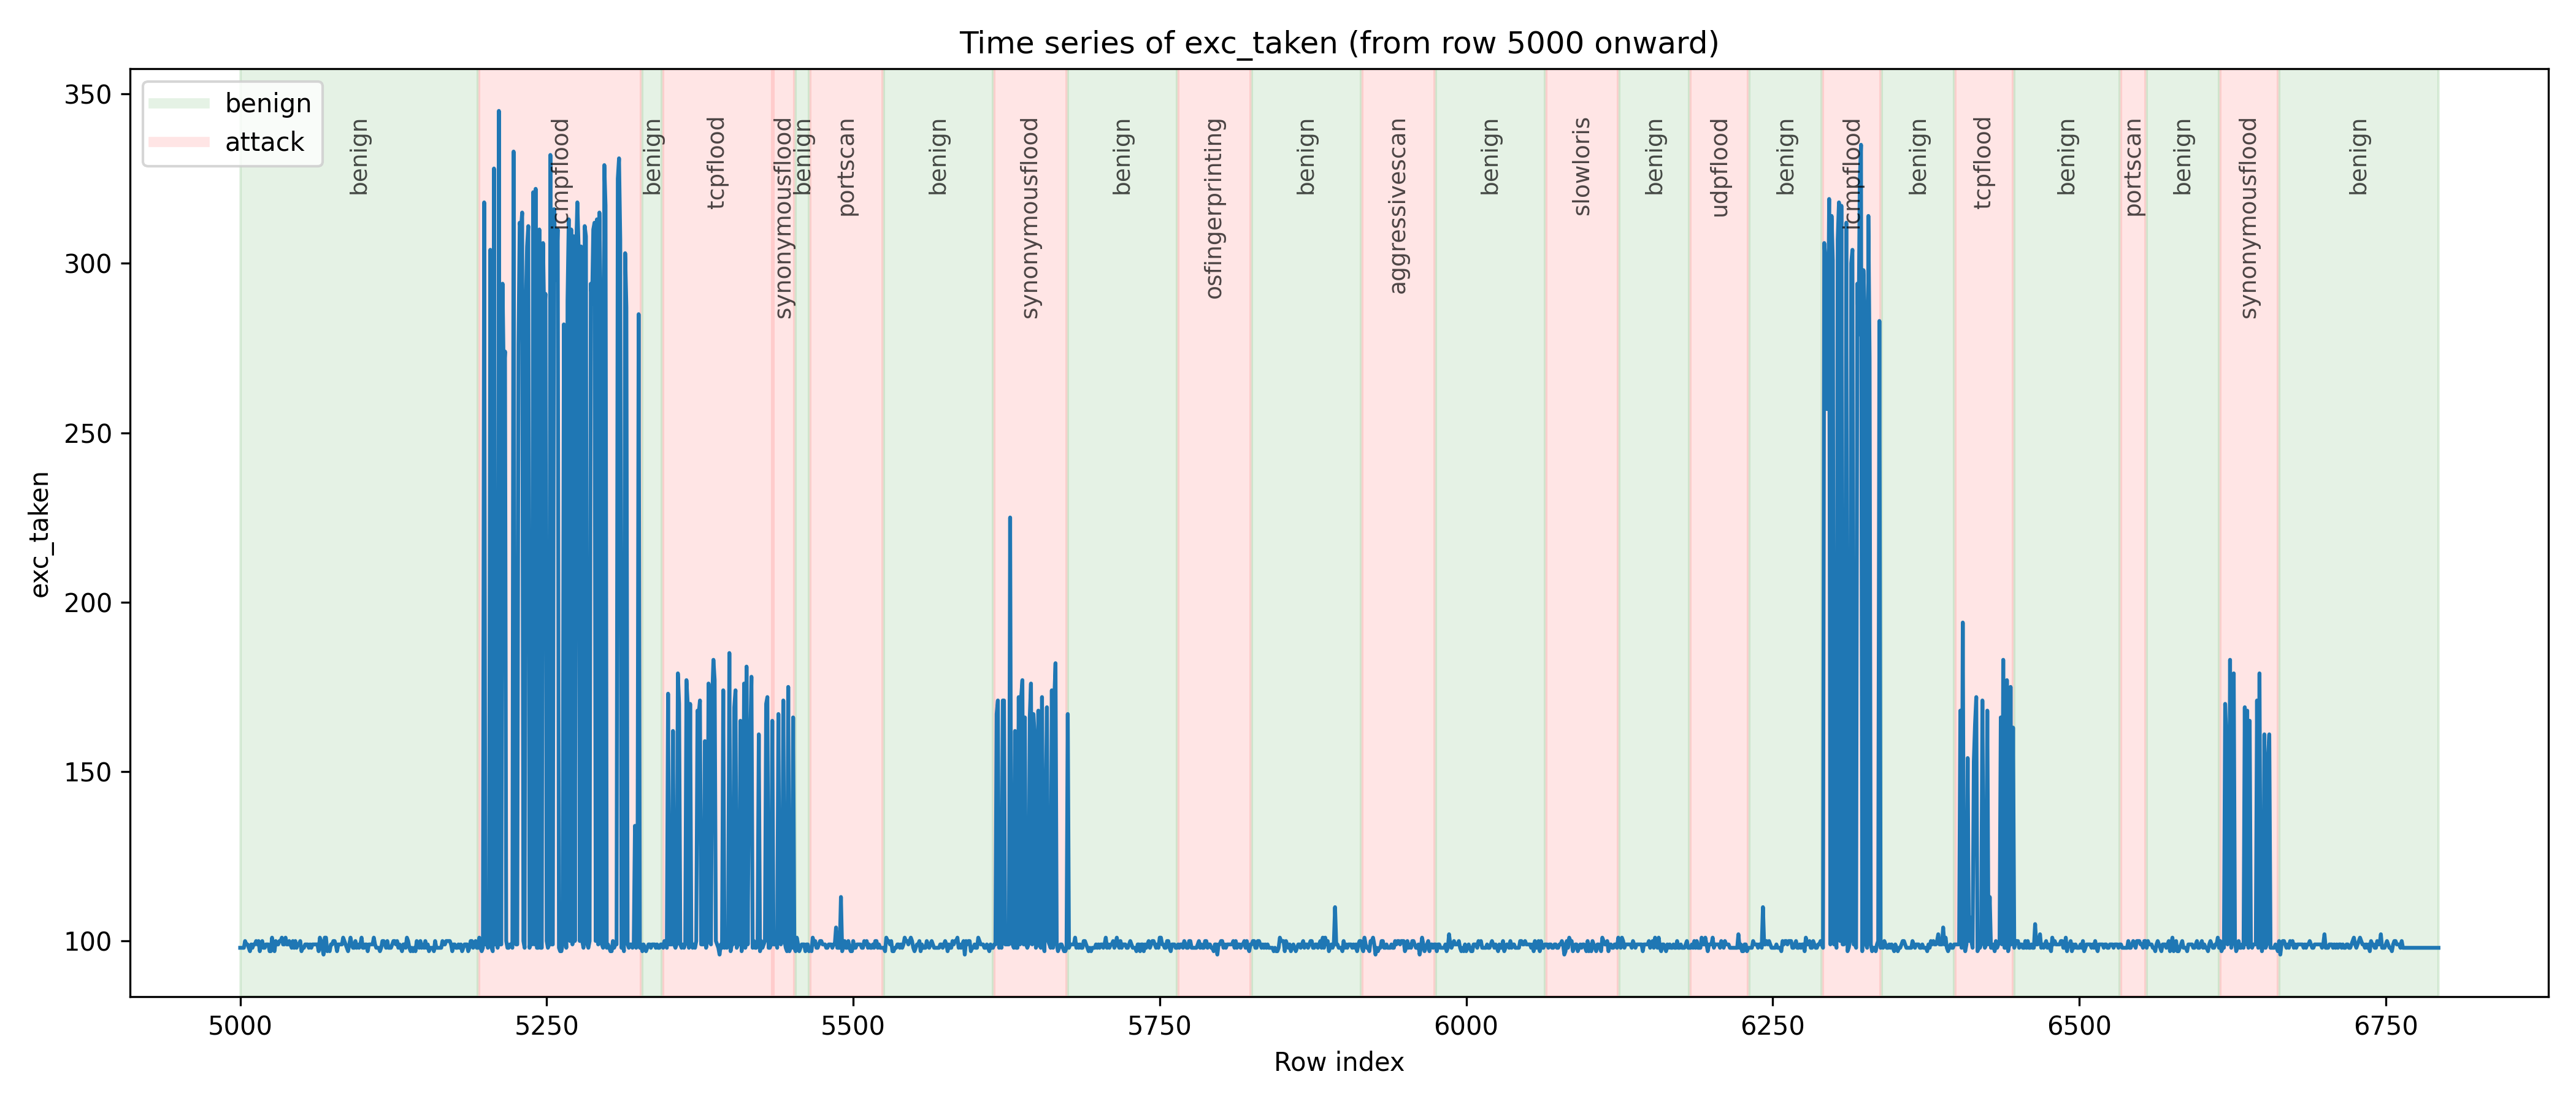
\includegraphics[width=1\textwidth]{pics/exc_taken.png}
  \vspace{-3mm} % Abstand manuell entfernen (anpassbar)
  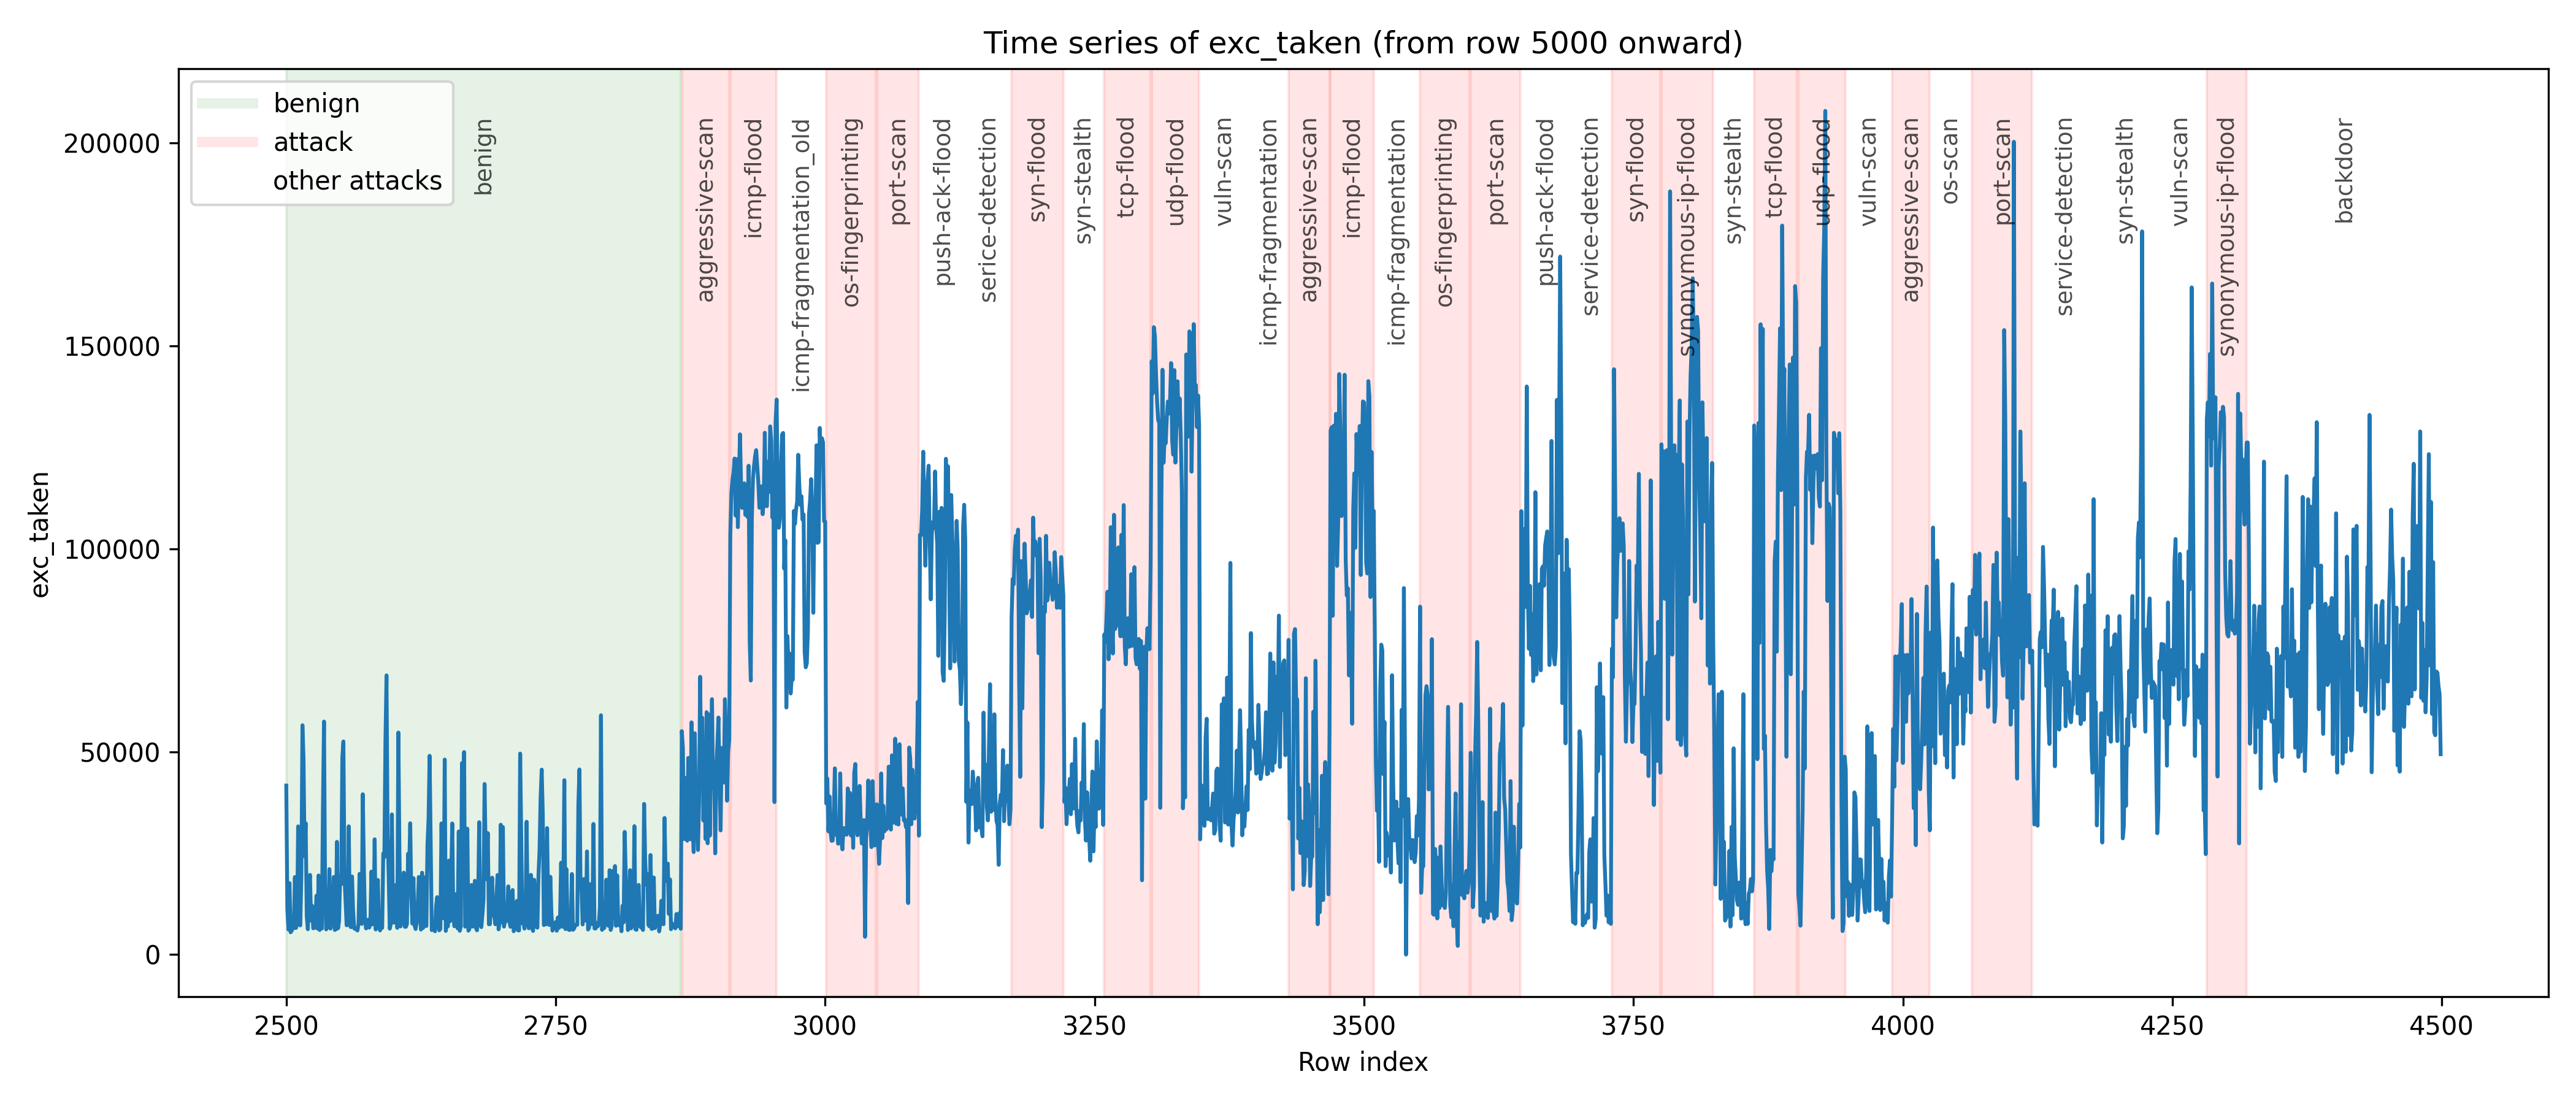
\includegraphics[width=1\textwidth]{pics/exc_taken_public.png}
  \caption{Comparison of \texttt{exc-taken} timelines: own dataset (top) and CICEVSE2024 dataset (bottom)}
  \label{fig:exc_taken_comparison}
\end{figure}
Despite notable differences in the absolute value ranges—likely due to architectural differences, sampling intervals, and system load—the time series of \texttt{exc\_taken} in both datasets exhibit structurally similar patterns. In both cases, this feature reacts to specific attacks with abrupt value changes especially by the flooding attacks are distinctive spikes, while maintaining stable behavior during benign phases. This confirms \texttt{exc\_taken} as a sensitive and transferable indicator of anomalous activity in kernel-space, suitable for machine learning-based intrusion detection approaches.
\begin{figure}[H]
  \centering
  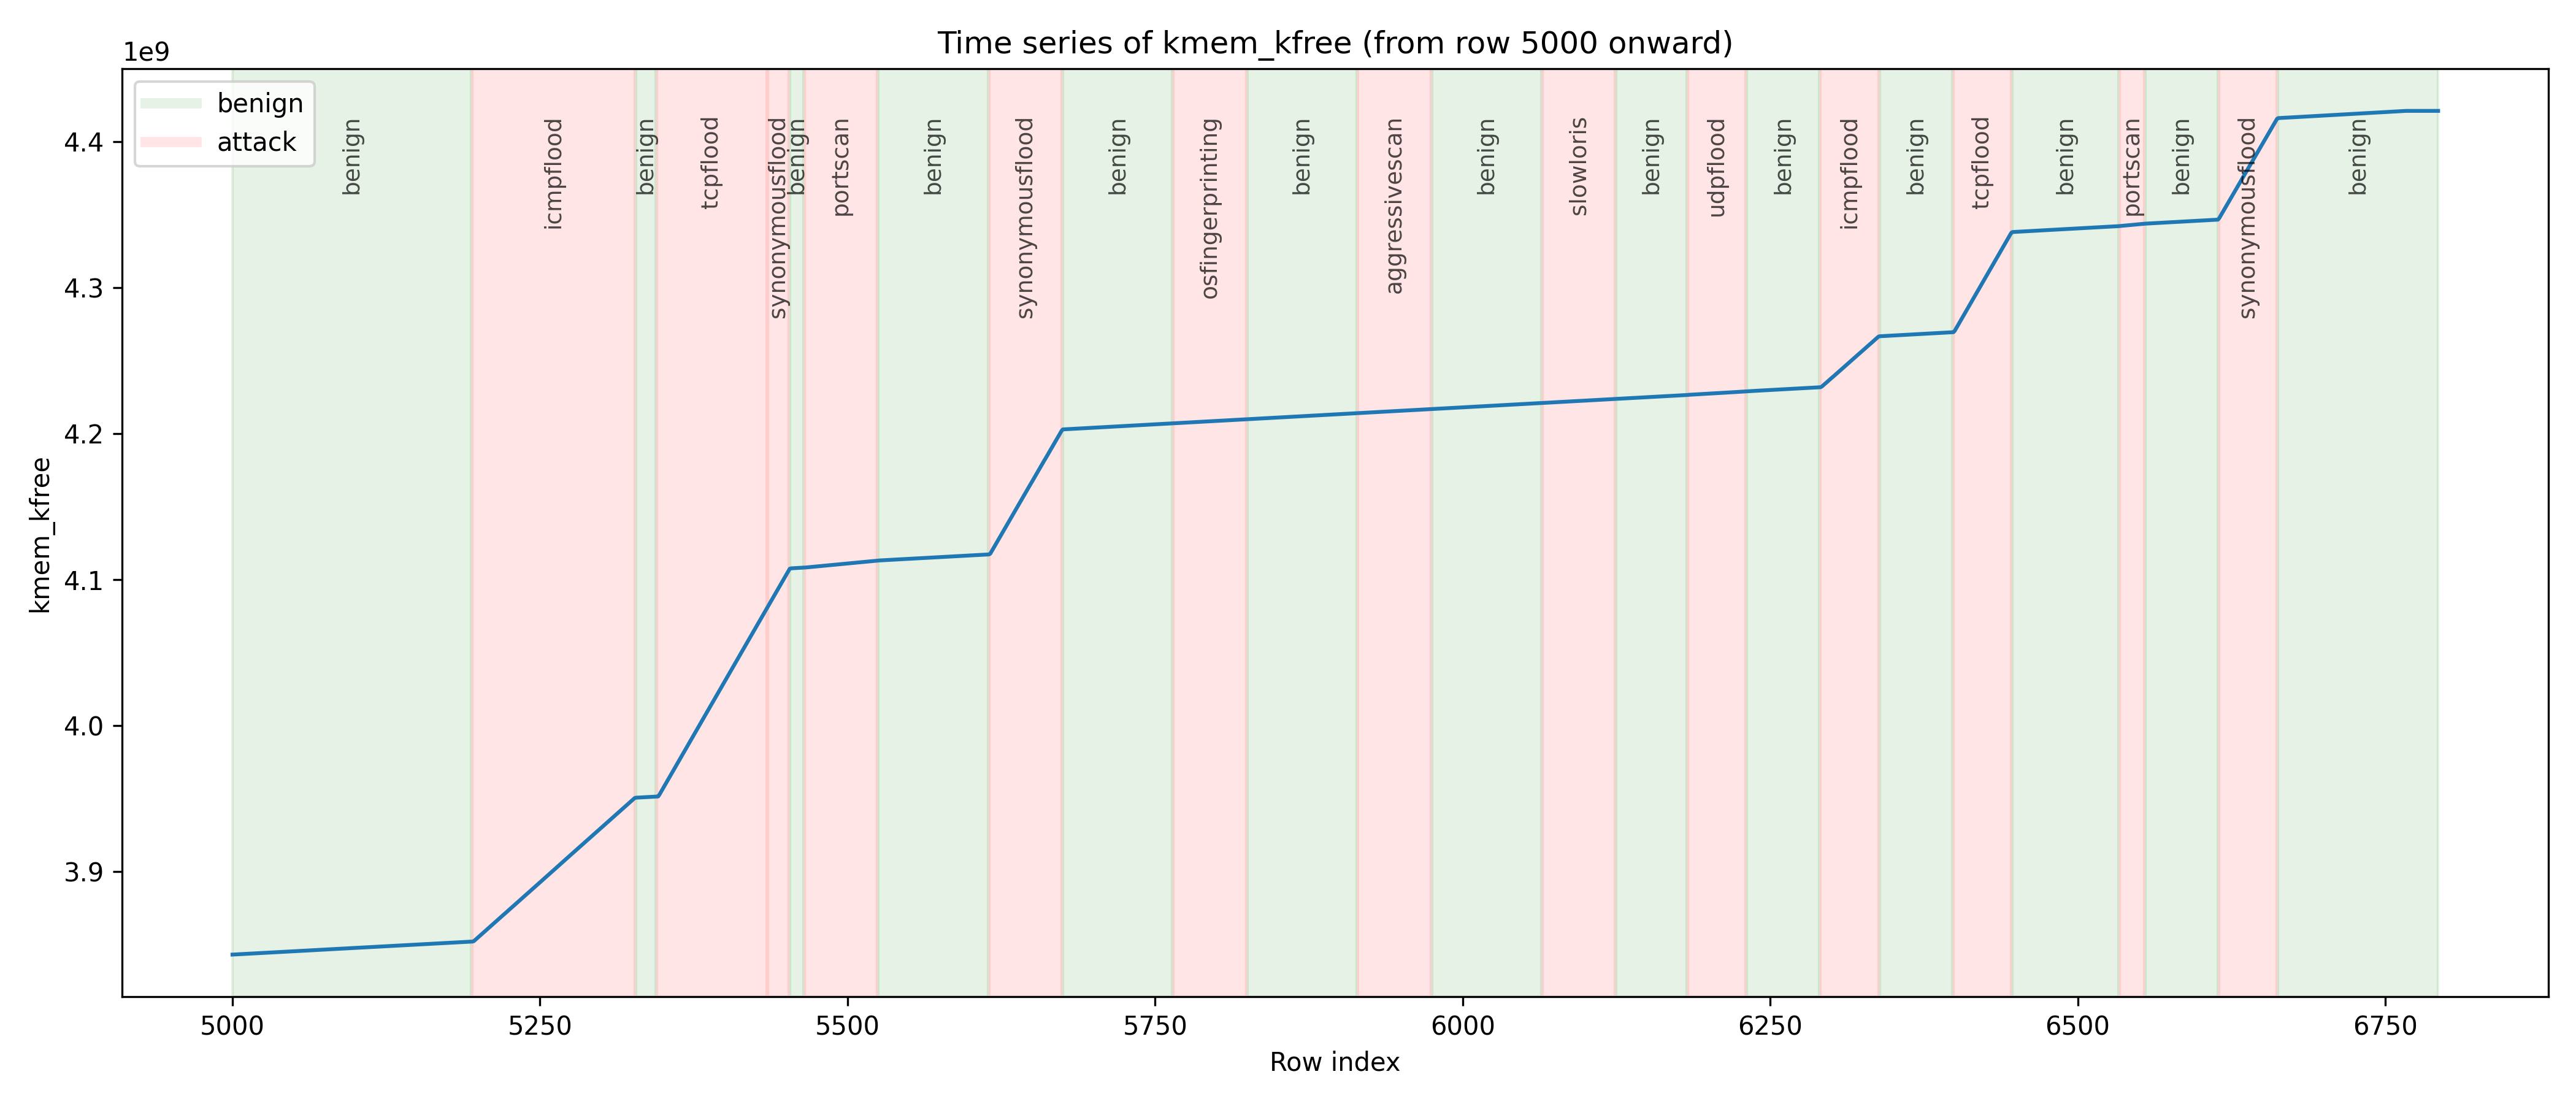
\includegraphics[width=1\textwidth]{pics/kmem_kfree.png}
  \vspace{-3mm} % Abstand manuell entfernen (anpassbar)
  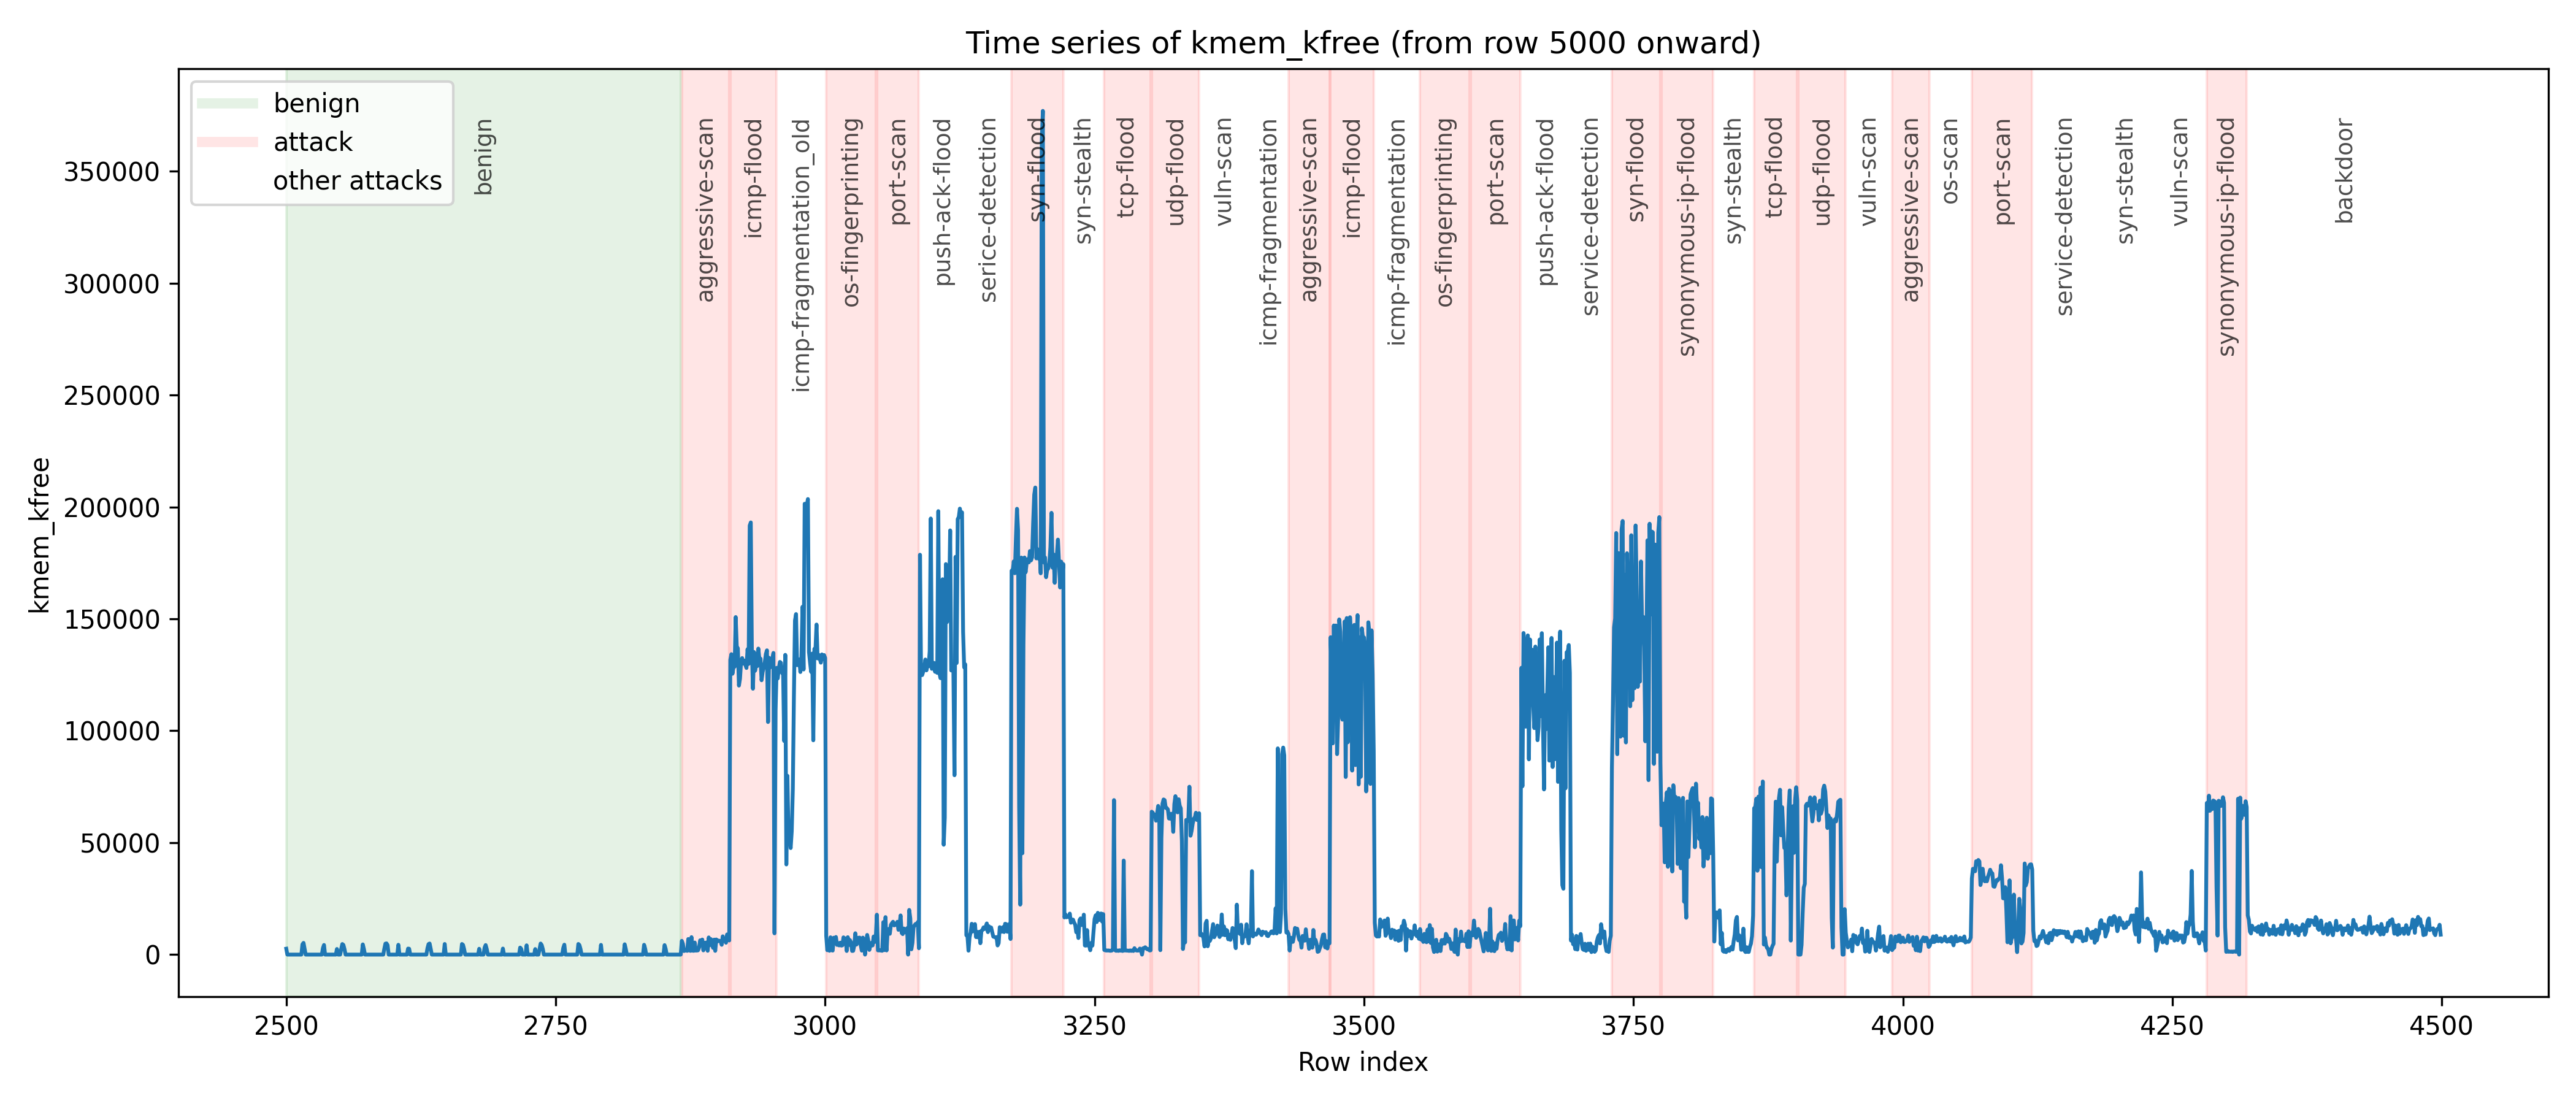
\includegraphics[width=1\textwidth]{pics/kmem_kfree_public.png}
  \caption{Comparison of \texttt{kmem-kfree} timelines: own dataset (top) and CICEVSE2024 dataset (bottom)}
  \label{fig:kmem_kfree_comparison}
\end{figure}
We observe similar peaks in both datasets, particularly during the flooding attacks, where the counter for \texttt{kmem\_kfree} increases noticeably. In our dataset, the resulting curve is cumulative, showing pronounced peaks corresponding to the attack phases. In contrast, the CICEVSE2024 dataset exhibits a more oscillating pattern, which is likely a result of different \texttt{perf} measurement flags. Specifically, their approach appears to monitor within a fixed time window, resetting the counter after each interval. This methodological difference leads to the observed oscillatory course in the public dataset, while the cumulative approach in our dataset amplifies peaks and produces a monotonically increasing curve.\\
\\
Therefore, we have sufficient data to train our models with minimal error values. Moreover, for the selected features from the paper \textit{Enhancing EV Charging Station Security Using a Multi-dimensional Dataset}~\cite{EV_Security}, we observe similar peaks and behavioral patterns in both attack and benign scenarios. This indicates a high degree of similarity between the datasets, further supporting the generalizability and validity of the selected features for anomaly detection.